\section{GLAM Simulations}\label{sec:glam}

Sec 2. Glam Section
Plot Glam with and without BAO measurements.
Describe Molino's covariance and put some justification. 1 Gpc cub.
Reference Jayashree's paper that the template works well for a range of redshifts. make a plot for sigma alpha vs kmax, with and without nuisance parameters.
Use CAMB to get the bao constraints for reconstructed power spectrum with GLAM parameters.

\begin{figure*}
\centering
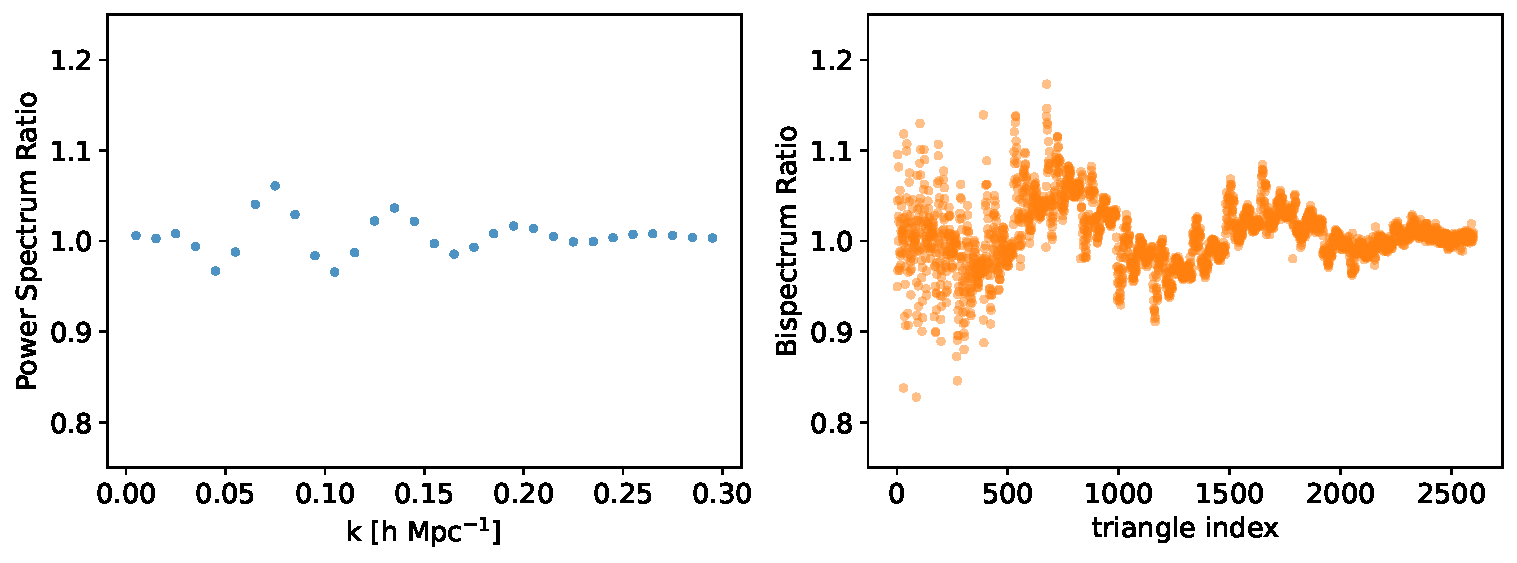
\includegraphics[width=0.95\textwidth]{glam_spec.pdf}
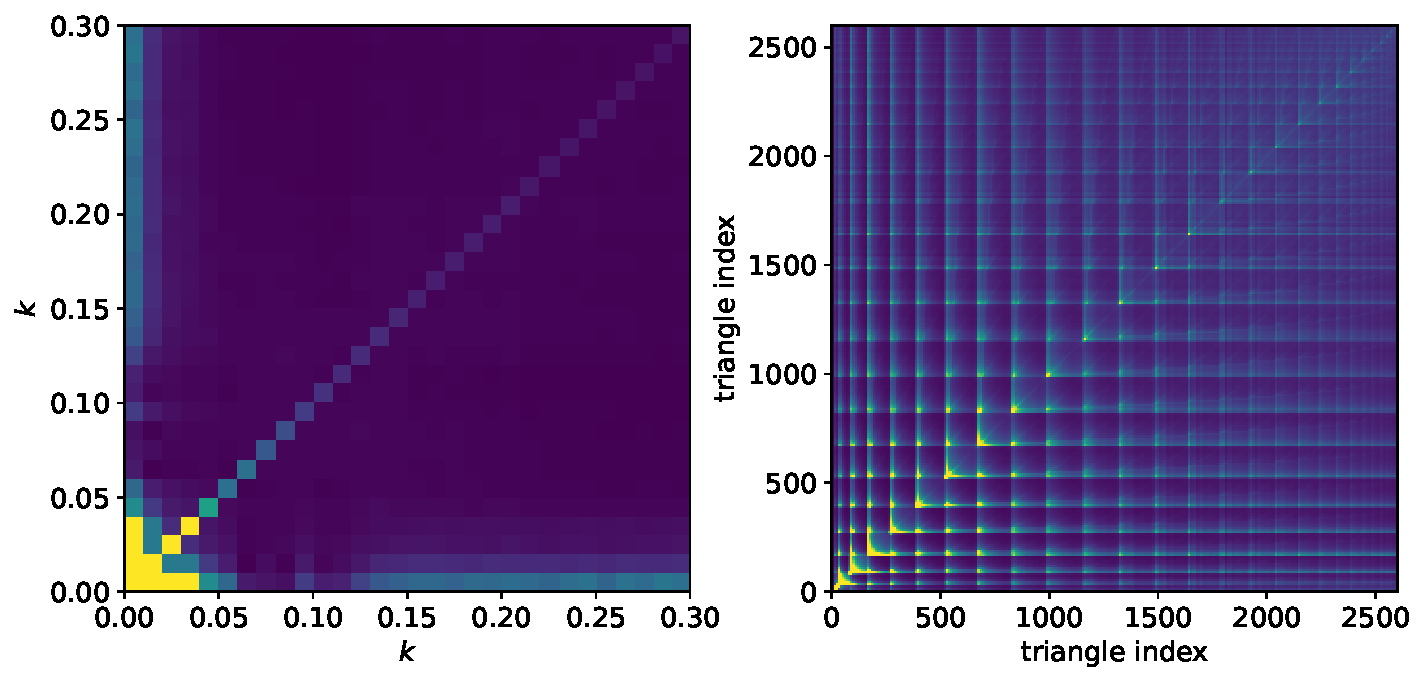
\includegraphics[width=0.95\textwidth]{glam_cov.pdf}
\caption{Mean power spectrum (bispectrum) of Glam mocks with BAO feature to that of the  mocks without BAO. Covariance matrices of Molino mocks normalized by Glam.}
\end{figure*}



\begin{figure}
\centering
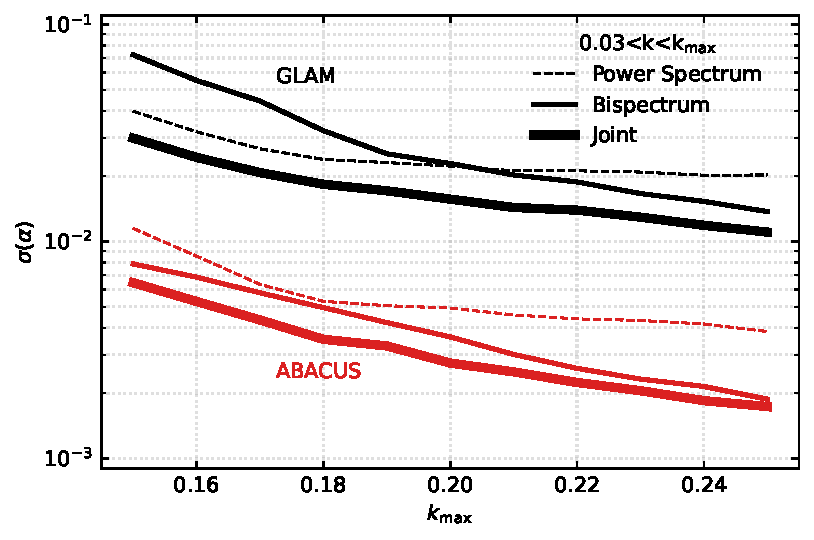
\includegraphics[width=0.45\textwidth]{sigma_kmax.pdf}
\caption{One sigma statistical uncertainty of BAO parameter $\alpha$ from Power Spectrum, Bispectrum, and Joint analysis.}
\end{figure}

Sec 3. BAO is DESI samples. Analyse Abacus mocks with template from Jayashree. Renormalize Molino's covariance by the ratio of spectra to get covariance for Abacus. Maybe use Glam and Molino to show that spectra ratio scales proportional to dispersion ratio.

Sec 4. BAO detection level. How well we can fit BAO with a smooth function. Mean Glam' with and without BAO as model 1 and 2, and mean Glam with BAO as data. Chi2 vs alpha.
